\section{Pre-study}
This section presents the project’s domain and describes how the domain is gradually refined into a 
problem statement through interviews and persona development. 
The work conducted in this phase corresponds to the empathize and define stages of the design thinking process\cite{DesignThinking}, 
with the goal of understanding users’ experiences, challenges, and needs before proposing any concrete solutions.

\subsection{Building understanding of the domain and users}
The initial draft for the project domain is defined broadly as enhancing learning outcomes in education. 
This broad framing was chosen deliberately in order to avoid premature narrowing of the problem space. 
By maintaining a wide domain at the beginning, it becomes possible to refine and specify the focus based 
on empirical insights rather than assumptions.

To better understand the domain, we have followed the guidelines for design thinking\cite{DesignThinking}, \textit{empathizing} with our user-base through conducting interviews both students and teachers across a wide range of
educational levels and ages.

Through these interviews we captured perceived challenges related to learning, motivation, and engagement in educational settings. These findings helped us in \textit{defining} our user-base and pain-points, and importantly, \textit{why} these are problems, helping us put this information into a broader context.

\subsection{Interview highlights}

Recurring themes were identified from interviews and personas. %TODO forbedre denne

\subsubsection{Students}
Several common themes emerged among students:
\begin{itemize}
    \item Social interaction plays an important role in motivation, a factor that became particularly evident during the COVID-19 period when digital teaching limited interaction.
    \item A feeling of accomplishment acts as a strong motivational driver.
    \item Students value the ability to engage with topics by asking questions and discussing with others, including teachers, peers, or digital tools such as large language models.
    \item AI tools are generally viewed positively, but there is limited guidance on how these tools should be used effectively.
    \item An imbalance between workload and assessment can lead either to fatigue (too many assignments and tests) or disengagement (too much freedom and lack of structure).
\end{itemize}

\subsubsection{Teachers}
Teachers highlighted a different but related set of challenges:
\begin{itemize}
    \item It is difficult to make teaching accessible to all students due to large variation in background, skills, and prior knowledge.
    \item Motivation is perceived as a major challenge among students.
    \item Making teaching enjoyable has become increasingly difficult in recent years.
    \item At higher educational levels, it is harder to establish personal contact with students, and lecturers often have greater responsibility for curriculum design.
    \item Large curricula limit opportunities for varied teaching methods, such as practical work, despite such methods being seen as beneficial for engagement.
\end{itemize}

Potential solutions are not defined at this stage. 
Instead, the focus remains on understanding the motivations behind the identified challenges. 
These motivations may later be addressed during ideating, prototyping and focusing phases.

\subsection{Building Personas}
Based on the interview data, three personas were developed from a total of seven interviews. 
The personas represent key user groups and capture common patterns in experiences, motivations, and challenges. 
These personas are included in the appendix and are used as analytical tools throughout the project to ensure 
that subsequent design decisions remain grounded in user needs.

\subsection{Domain Models}
\begin{figure}[H]
    \centering
    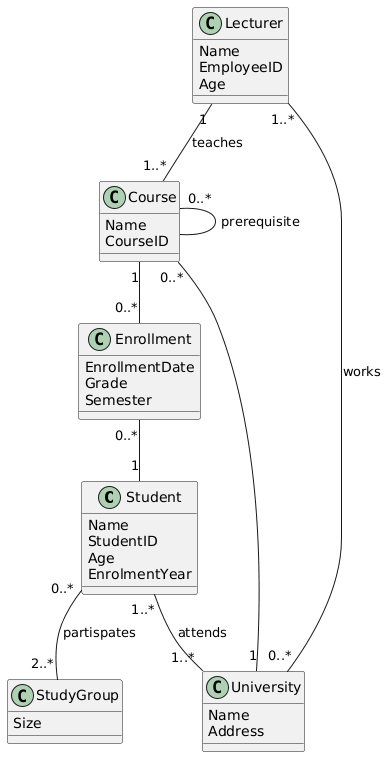
\includegraphics[width=0.7\textwidth]{images/domainModel}
    \caption{Domain model of the system showing relationships between students, courses, lecturers, and study groups.}
    \label{fig:domain-model}
\end{figure}
The current domain model Figure \ref{fig:domain-model} includes the entities \textit{Lecturer}, \textit{Course},
\textit{Enrollment}, \textit{Student}, \textit{StudyGroup}, and \textit{University}.
Relationships have been modeled with multiplicities in order to clarify how these entities connect to one another.
Examples include lecturers teaching courses, students enrolling in courses, students participating in study groups, and students attending a university.

This domain model captures many of the structural and administrative elements of the academic environment.
It shows how students, lecturers, courses, and institutions are connected, and it provides a foundation for modeling participation and organization within the system.

At the same time, the model also reveals a limitation in relation to the project's broader goal.
Since the system aims to support gamification of studying, it is not enough to model only the academic structure around the student.
The actual act of studying is not currently represented explicitly in the model.
For this reason, we considered whether it would be beneficial to add an entity such as \textit{StudySession}.
%TODO Fixe disse avsnittene
%TODO HUSK REF TIL DESCRIPTIVE AND PRESCRIPTIVE

A \textit{StudySession} entity could help represent studying as an activity rather than only as enrollment or membership.
This would make it easier to support features such as focus mode, streaks, participation feedback,
and progress tracking that are central to several of the user stories.
However, introducing such an entity also raises questions about detail: the group still needs to decide whether study
activity should be modeled in a simple way or whether finer-grained information is necessary.




\subsection{Design-Thinking Perspective}
In this pre-study we have followed the design thinking process \cite{DesignThinking}. The focus has primarily been on the early stages of design-thinking, namely empathizing
with the target demographic and transitioning this understanding toward defining specific problem characteristics.

\subsubsection{Empathizing}
As all group members have personal experience as students, it was important to acknowledge and actively mitigate potential bias. 
The goal was to understand the problem from the perspective of the interview participants rather than relying on personal assumptions. 
Both teachers and students indicated that the educational context has changed in recent years, particularly following the 
COVID-19 pandemic and the increased presence of AI tools.

To capture these perspectives, the interviews emphasized exploratory questions focused on underlying reasons and experiences.
Asking “why” questions helped elicit deeper insights into participants’ motivations, challenges, and perceptions.

\subsubsection{Define}
To catch a broad perspective of our problem domain, we searched for diversity among our interview subjects.
Students differed in age, motivation, and learning preferences, 
while teachers operated in highly diverse contexts, ranging from primary education to university level teaching. 
To move toward a more concrete problem formulation, common challenges were identified across interviews and synthesized into personas.

These personas serve as abstractions of key user groups and help clarify the core problems within the domain. 
Throughout the project, they will be used to evaluate and validate proposed ideas and prototypes, ensuring alignment with the needs of the target demographic.

\subsubsection{Ideation}
Based on the results of empathizing and defining phases, we were now ready to decide on a specific target demographic and problem domain.
As a result from our group's brainstorming, we settled on focusing on university students and improving motivation and social attendance through gamification.
\begin{figure}[H]
    \centering
    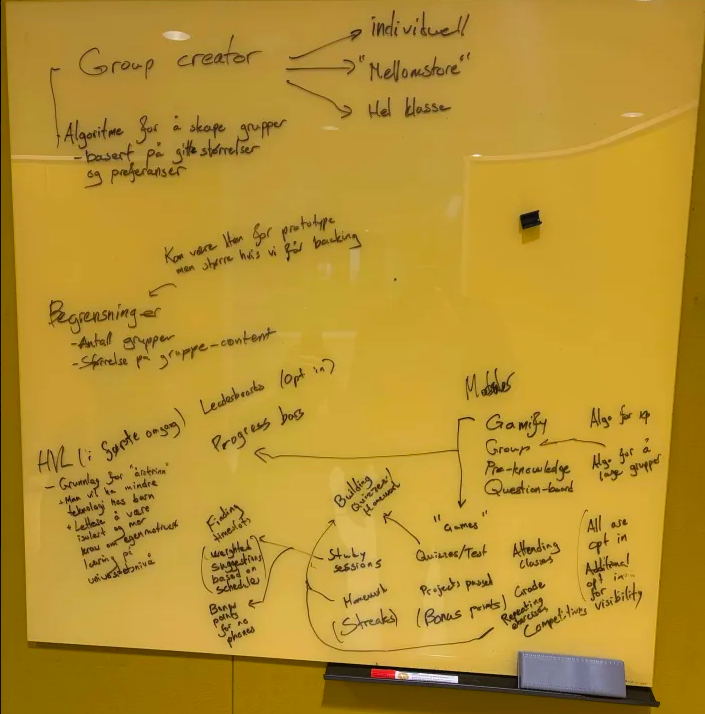
\includegraphics[width=0.5\linewidth]{images/brainstorming.png}
    \caption{The resulting artifact from our brainstorming session}
    \label{brainstorming}
\end{figure}

This concludes the parts of design-thinking relevant to the pre-study section of this report. Later on in the report we will further elaborate on our experiences with the cycles of prototyping and testing.

\subsection{Context and Design Science}
The pre-study addresses a relevant real world problem faced by university students, including challenges related to 
understanding course material, maintaining motivation, and coping with academic pressure in a largely self directed 
learning environment.
In accordance with Hevner’s design science framework\cite{DesignScience}, the project environment was explored
through interviews, persona development, and domain modeling to ensure problem relevance.

Although no final system has been developed at this stage, the pre-study has produced several design artifacts, such 
as personas and domain models, which contribute to understanding the problem space and guiding future design decisions. 
The project is planned to follow an iterative build--reflect process, where insights from user feedback continuously refine 
the design, reflecting Hevner’s view of design as a search process\cite{DesignScience}.

Overall, the project emphasizes utility and practical impact rather than theory building, which aligns with the goals of 
design science research.
The final report is intended to be accessible both to students and administrators, as well as to
a more technology-oriented audience.

\subsection{Abstraction Reflection}
% TODO: Change order here or rewrite..
At the start of the project, the group struggled with abstraction by prematurely committing to a concrete solution. 
The initial idea was to develop a system that gamifies studying. 
After discussing this approach with the course 
instructor, it became clear that the focus needed to shift away from implementation and toward understanding the underlying problem.

As described by Kramer\cite{AbstractionKey}, poor abstraction often leads to solutions that replicate complexity or address surface level symptoms rather than capturing the essence of a problem. 
In response, we refocused on identifying and abstracting 
the core challenges within the domain. 
Structured interviews were conducted to explore why students and teachers experience 
difficulties related to motivation, engagement, and learning.

This process required removing solution specific assumptions and instead generalizing across interview data to identify 
recurring patterns and needs. 
In line with Kramer’s discussion\cite{AbstractionKey}, this transition represented a move from concrete thinking 
toward a more abstract problem formulation, emphasizing an understanding of what the problem is before determining how it 
should be addressed. 
This experience reinforced the importance of abstraction as a prerequisite for developing production 
designs that are both meaningful and fit for purpose.



